\begin{figure}[htp]
	\centering\capstart
	\subfloat[\(\Re{\pixel{\mathcal{SG}}}\)]{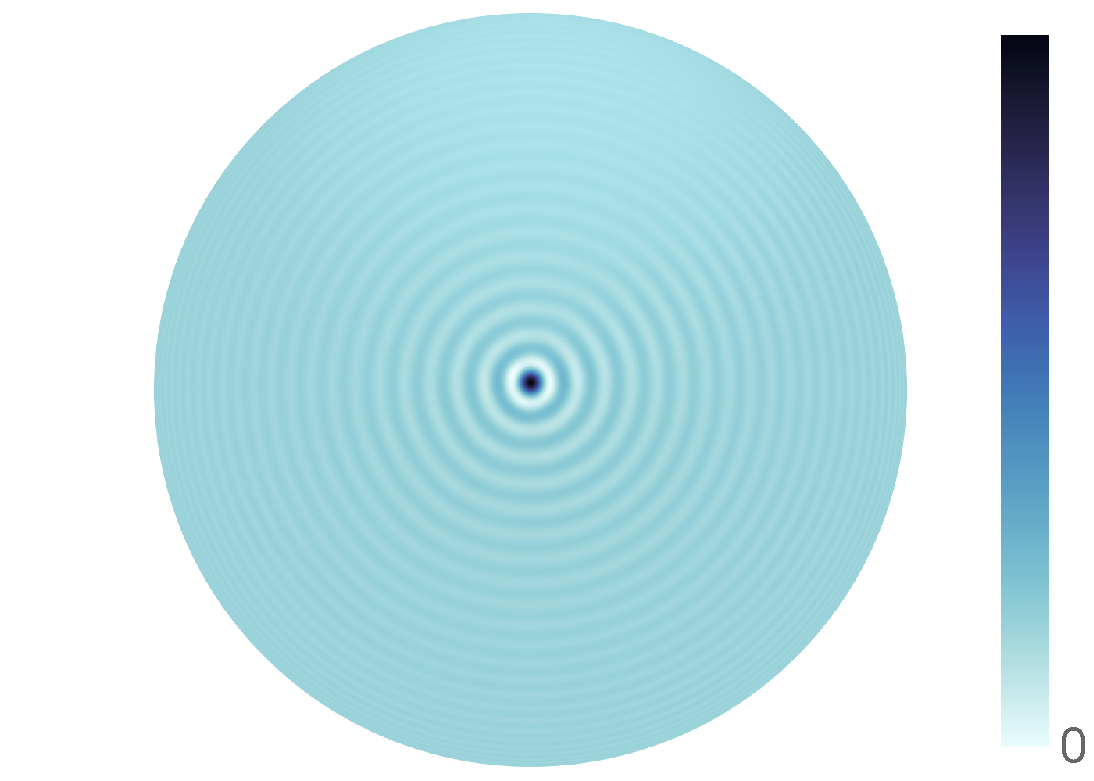
\includegraphics[trim={23 7 3 6},clip,width=.5\textwidth]{squashed_gaussian_1tsig100_1freq10_L128_res512_real_norm.pdf}}
	\hfill
	\subfloat[\(\Re{\pixel{(\translation{\omega'}\mathcal{SG})}}\)]{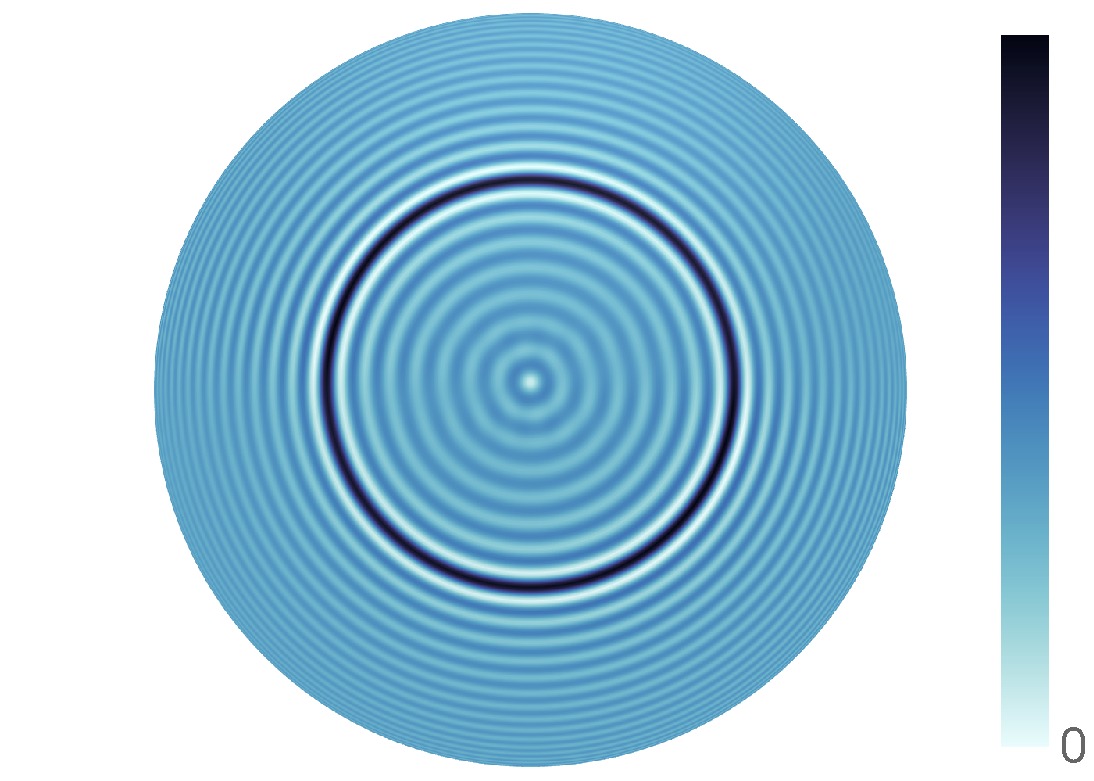
\includegraphics[trim={23 7 3 6},clip,width=.5\textwidth]{squashed_gaussian_1tsig100_1freq10_L128_translate_alpha3pi4_beta1pi8_res512_real_norm.pdf}}
	\caption[
		A squashed Gaussian at the north pole and then translated
	]{
		Panel (a) presents the squashed Gaussian (bandlimited at \(L=128\)).
		The squashed Gaussian is then translated to some \(\omega'=(\theta',\phi')\), as shown in panel (b).
		The odd azimuthal symmetry in the initial kernel definition is preserved under translation.
		The colour is between zero and one, reflecting the scaled intensity of the field.
	}\label{fig:chapter2_squashed_gaussian}
\end{figure}
